\chapter{Análisis comparativo}

\section{Teoría previa}
\subsection{Índices de rendimiento}
\begin{itemize}
    \item \textbf{CPI}
    \[
    \text{CPI}=\dfrac{\text{Ciclos}}{\text{Instruccion}}
    \]
    \item \textbf{MIPS}
    \[
    \text{MIPS}=
    \dfrac{\text{Nº Instrucciones}}{\text{T. ejecución} \cdot 10^6}=
    \dfrac{\text{Freq de reloj}}{\text{CPI} \cdot 10^6}
    \]
    \item \textbf{MFLOPS}
    \[
    \text{MFLOPS}=
    \dfrac{\text{Nº instrucciones FP}}{\text{T. ejecución} \cdot 10^6}
    \]
\end{itemize}
\subsection{¿Cómo expresar el rendimiento?}
\begin{itemize}
    \item \textbf{Media aritmética}
    \[
    x_a = \dfrac{1}{n}\sum_{i=1}^n x_i
    \]
    \item \textbf{Media armónica}
    \[
    x_f = \dfrac{n}{\sum_{i=1}^n \frac{1}{x_i}}
    \]
    \item \textbf{Media geométrica}
    \[
    x_g = (\prod_{i=1}^n x_i)^\frac{1}{n}
    \]
\end{itemize}
\subsection{Diferencias estadísticamente significativas}
\begin{figure}[H]
    \centering
    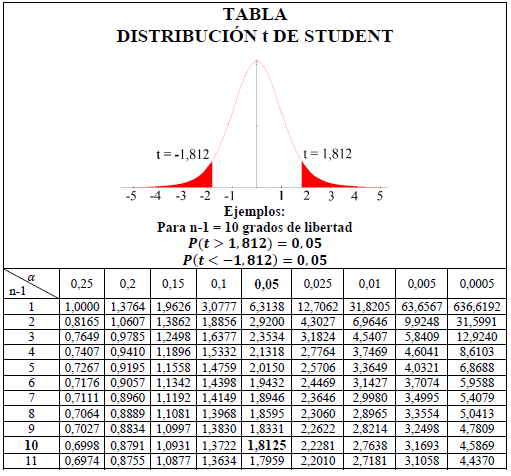
\includegraphics[width=0.9\textwidth]{Images/tabla-t.png}
\end{figure}
Supongamos la ejecución de n programas en dos máquinas A y B. ¿Son significativas las diferencias obtenidas? Para saberlo utilizamos el intervalo de confianza:

\begin{equation}
\Large
\bar{x} \pm t_{1-\frac{\alpha}{2},n-1} \cdot \dfrac{s}{\sqrt{n}}
\end{equation}
Donde:\begin{itemize}
    \item \textbf{$t$} es el valor obtenido de la tabla T-student.
    \item \textbf{$s$} es la desviación típica.
    \item \textbf{$\alpha$} es el nivel de confianza.
\end{itemize}
\newpage
\section{Ejercicios resueltos}
\subsection{Ejercicio 1}
\noindent
Un programa ejecuta un total de $120\times 10^6$instrucciones. De ellas, el 75\% se ejecutan en 3 ciclos de reloj, mientras que el resto lo hace en 5 ciclos. Tras medir el tiempo de ejecución de este programa mediante la orden time del sistema operativo se ha obtenido la siguiente información:
\begin{lstlisting}[language=C]
real 0m84s
user 0m34s
sys 0m1s
\end{lstlisting} 
Calcular el número medio de ciclos por instrucción (CPI) obtenidos por el programa, la frecuencia del procesador y los MIPS.
\begin{tcolorbox}[colback=white,colframe=cyan!50!black,fonttitle=\bfseries]
\[120\cdot 10^6\left.\begin{array}{ll}
\fd 75\%\fd 3\quad\text{ciclos}\\
\fd 25\%\fd 5\quad\text{ciclos}
\end{array}\right.
\]
\[
\text{CPI}=\dfrac{(3\cdot0.75\cdot 120\cdot 10^6)+(5\cdot 0.25\cdot 120\cdot 10^6)}{120\cdot 10^6}=3\cdot 0.75+5\cdot 0.25=3.5
\]
\[
\text{CPI}=\dfrac{T_{\text{ej}\cdot F_q}}{\text{NºI}}\fd F_q=\dfrac{\text{CPI}\cdot\text{NºI}}{T_{\text{ej}}}\fd F_q=\dfrac{\text{CPI}\cdot\text{NºI}}{T_{\text{ej}}}=\dfrac{3.5\cdot 120\cdot 10^6}{(34+1)}=12\text{Mhz}
\]
\[
\text{MIPS}=\dfrac{F_q}{\text{CPI}\cdot 10^6}=3.42
\]
\end{tcolorbox}
\subsection{Ejercicio 2}
\noindent
Un estudio llevado a cabo mediante un monitor de ejecución de programas ha permitido cuantificar el tiempo medio de ejecución de las instrucciones que emplea una aplicación informática. Esta aplicación se ha ejecutado en dos procesadores P y Q, con el mismo juego de instrucciones y se ha obtenido el siguiente resultado:
\begin{table}[H]
\centering
\scalebox{0.7}{\begin{tabular}{|c|c|c|c|}
\hline
\textbf{Tipo de Instrucción} & \textbf{Frecuencia en \%} & \textbf{Tiempo en P en ns} & \textbf{Tiempo en Q en ns} \\ \hline
Memoria                      & 25                        & 70                         & 72                         \\ \hline
Comparación                  & 35                        & 32                         & 27                         \\ \hline
Salto                        & 25                        & 13                         & 10                         \\ \hline
Otras                        & 15                        & 18                         & 12                         \\ \hline
\end{tabular}}
\end{table}
\begin{enumerate}
    \item Calcular el tiempo medio de ejecución de una instrucción en cada procesador y utilizar el resultado para cuantificar la mejora conseguida por el procesador más rápido.
\begin{tcolorbox}[colback=white,colframe=cyan!50!black,fonttitle=\bfseries]
\[\left.\begin{array}{ll}
TP=0.25\cdot 70+0.35\cdot32+0.25\cdot 13+0.15\cdot 18=34.65\\
TQ=0.25\cdot 72+0.35\cdot 27+0.25\cdot 10+0.15\cdot 12=31.75
\end{array}\right.
\]
\[
\text{ratio}=\dfrac{TP}{TQ}=1+\dfrac{9.13}{100}
\]
Q es 9.13 veces más rápido que R.
\end{tcolorbox}    
    \item Determinar el nuevo tiempo medio de ejecución de una instrucción en el procesador si un nuevo diseño consigue que todas las instrucciones se ejecuten un 15\% más rápidamente.
\begin{tcolorbox}[colback=white,colframe=cyan!50!black,fonttitle=\bfseries]
\[
T_{\text{mej}}R=\dfrac{34.65}{1.15}=30.13
\]
\[
T_{\text{mej}}Q=\dfrac{31.75}{1.25}=27.60
\]
\end{tcolorbox}    
\end{enumerate}
\subsection{Ejercicio 3}
\noindent
Considérese un programa de cálculo numérico que se ejecuta en dos minutos y hace las operaciones de coma flotante que se indican en la tabla ¿Cuál es el rendimiento conseguido por el computador con este programa de cálculo atendiendo a los MFLOPS? ¿Y con los MFLOPS normalizados?
\begin{table}[H]
\centering
\begin{tabular}{|c|c|c|}
\hline
\textbf{Operación} & \textbf{Cantidad} & \textbf{Operaciones normalizadas} \\ \hline
ADD                & $78\times10^6$            & 1                                 \\ \hline
SQRT               & $29\times10^6$            & 3                                 \\ \hline
COS                & $13\times10^6$            & 8                                 \\ \hline
EXP                & $42\times10^6$            & 12                                \\ \hline
\end{tabular}
\end{table}
\begin{tcolorbox}[colback=white,colframe=cyan!50!black,fonttitle=\bfseries]
Sin normalizar:
\[
\text{MFLOPS}=\dfrac{\text{nº inst}}{t\cdot 10^6}=\dfrac{120}{160}=1.35\text{MFLOPS}
\]
Normalizado:
\[
\text{MFLOPS}=\dfrac{78\cdot 10^6+29\cdot 10^6\cdot 3+13\cdot 10^6\cdot 8+42\cdot 10^6\cdot 12}{120\cdot 10^6}=6.442\text{MFLOPS}
\]
\end{tcolorbox}
\subsection{Ejercicio 4}
\noindent
El rendimiento de un programa que implementa un algoritmo numérico varía de acuerdo con las distintas secciones de código. En concreto, la generación de resultados del algoritmo se distribuye de acuerdo con los siguientes MFLOPS:
\begin{table}[H]
\centering
\begin{tabular}{|c|c|}
\hline
\textbf{Porcentaje de resultados} & \textbf{MFLOPS} \\ \hline
30\%                              & 1               \\ \hline
20\%                              & 10              \\ \hline
50\%                              & 100             \\ \hline
\end{tabular}
\end{table}
\noindent
Calcular el valor medio de los MFLOPS obtenidos por el algoritmo ¿Cómo se distribuye el tiempo de ejecución en función de los MFLOPS?
\begin{tcolorbox}[colback=white,colframe=cyan!50!black,fonttitle=\bfseries]
\[
x=\dfrac{1}{\sum\dfrac{wi}{xi}}
\]
\[
\dfrac{1}{\dfrac{0.3}{1}+\dfrac{0.2}{10}+\dfrac{0.5}{100}}=3.08\text{MFLOPS}
\]
\[
30\%\fd\dfrac{0.3}{0.325}=0.923\fd 92.3\%\quad\text{se ejecuta 1MFLOP}
\]
\[
20\%\fd\dfrac{0.02}{0.325}=0.062\fd 6.2\%\quad\text{a 10 MFLOP}
\]
\[
50\%\fd\dfrac{0.005}{0.325}=0.015\fd 1.5\%\quad\textbf{a 100 MFLOPS}
\]
\end{tcolorbox}
\subsection{Ejercicio 5}
\noindent
Calcula los índices de rendimiento SPEC int\_base2000 y SPECint2000 de los sistemas A y B a partir de las siguientes medidas:
\begin{table}[H]
\centering
\scalebox{0.7}{\begin{tabular}{|c|c|c|c|c|c|}
\hline
\textbf{Programa} & \textbf{\begin{tabular}[c]{@{}c@{}}Referencia\\ (Base \& Peak)\end{tabular}} & \textbf{\begin{tabular}[c]{@{}c@{}}A Base Run\\ Time\end{tabular}} & \textbf{\begin{tabular}[c]{@{}c@{}}A Peak Run\\ Time\end{tabular}} & \textbf{\begin{tabular}[c]{@{}c@{}}B Base Run\\ Time\end{tabular}} & \textbf{\begin{tabular}[c]{@{}c@{}}B Peak Run\\ Time\end{tabular}} \\ \hline
P1                & 2100                                                                         & 456                                                                & 440                                                                & 420                                                                & 415                                                                \\ \hline
P2                & 2400                                                                         & 792                                                                & 780                                                                & 810                                                                & 805                                                                \\ \hline
P3                & 3200                                                                         & 820                                                                & 796                                                                & 816                                                                & 715                                                                \\ \hline
\end{tabular}}
\end{table}
\noindent
\textbf{Observación}: SPECint\_base2000 (SPECint2000) se calcula como 100 x MediaGeométrica(ratios Ri/Ti) siendo Ri el valor de referencia y Ti el valor de Base Run Time (Peak Run Time).
\begin{tcolorbox}[colback=white,colframe=cyan!50!black,fonttitle=\bfseries]
Media geométrica:
\[
X_t=\sqrt[n]{\prod_1^n xi}=\prod_1^n xi^{\dfrac{1}{w}}
\]
A$_{\text{base}}\fd x_1=\dfrac{210}{456}=4.61$; $x_2=\dfrac{2500}{792}=3.02$; $x_3=\dfrac{3200}{820}=3.9$; $n=3$.\\
Solución A$_{\text{base}}=\text{SPEC}_A=100\cdot\sqrt[B]{4.61\cdot 3.02\cdot 3.9}=100\cdot\sqrt{4.61\cdot 3.02\cdot 3.9}$\\
$\text{SPEC}_B=100\cdot\sqrt[3]{58.03}>100\sqrt[3]{54.29}$\\
B es mejor que A.
\end{tcolorbox}
\subsection{Ejercicio 6}
\noindent
Calcula los MFLOPS promedio de un sistema a partir de la siguiente tabla, que muestra el tiempo de ejecución y el número de operaciones de coma flotante de cuatro programas:
\begin{table}[H]
\centering
\begin{tabular}{|c|c|c|}
\hline
\textbf{Programa} & \textbf{Tiempo (s)} & \textbf{Operaciones} \\ \hline
P1                & 878                 & $230\times10^9$               \\ \hline
P2                & 491                 & $210\times10^9$               \\ \hline
P3                & 375                 & $151\times10^9$               \\ \hline
P4                & 427                 & $120\times10^9$               \\ \hline
\end{tabular}
\end{table}
\begin{tcolorbox}[colback=white,colframe=cyan!50!black,fonttitle=\bfseries]
\[\left.\begin{array}{llll}
P1=\dfrac{230\cdot 10^9}{878\cdot 10^6}=267\\\\
P2=\dfrac{210\cdot 10^9}{491\cdot 10^6}\\\\
P3=\dfrac{151\cdot 10^9}{375\cdot 10^6}\\\\
P4=\dfrac{120\cdot 10^9}{427\cdot 10^6}
\end{array}\right.
\]
\[
\text{MFLOPS}(P1,P2,P3,P4)=\dfrac{(230+210+150+120)\cdot 10^9}{(878+491+575+427)}=327.5\text{MFLOPS}
\]
\[
X_H=\dfrac{4}{\dfrac{1}{267}+\dfrac{1}{P2}+\dfrac{1}{P3}+\dfrac{1}{P4}}=328\text{MFLOPS}
\]
\end{tcolorbox}
\subsection{Ejercicio 7}
\noindent
La página oficial de SPEC muestra los siguientes resultados de rendimiento para dos sistemas informáticos obtenidos mediante el benchmark CPU2000:
\begin{table}[H]
\centering
\begin{tabular}{|c|c|c|c|}
\hline
\textbf{Sistema} & \textbf{Modelo}               & \textbf{SPECint\_base} & \textbf{SPECint2000} \\ \hline
A                & Altos G5350 (AMD Opteron 246) & 1347                   & 1438                 \\ \hline
B                & Altos G5350 (AMD Opteron 254) & 1788                   & 1918                 \\ \hline
\end{tabular}
\end{table}
\begin{enumerate}
    \item ¿Cuál de los dos sistemas presenta mejor rendimiento? Cuantifique numéricamente la mejora.
\begin{tcolorbox}[colback=white,colframe=cyan!50!black,fonttitle=\bfseries]
\[
\text{SPEC}_{\text{int}}\_\text{base2000}=\dfrac{1788}{1347}
\]
\[
\text{SPECint2000}=\dfrac{1918}{1438}
\]
\end{tcolorbox}    
    \item A la vista de los resultados anteriores, ¿afecta al rendimiento de ambos sistemas la optimización realizada por el compilador en las pruebas?
\begin{tcolorbox}[colback=white,colframe=cyan!50!black,fonttitle=\bfseries]
\[
\dfrac{\text{max}}{\text{min}}=7.2\%\quad\text{mejor con optimización}
\]
\end{tcolorbox}    
    \item ¿En qué medida se reflejará en los resultados anteriores una mejora importante en la unidad de coma flotante del procesador?
\begin{tcolorbox}[colback=white,colframe=cyan!50!black,fonttitle=\bfseries]
Los índices SPEC solo se basan en aritmética entera.
\end{tcolorbox}    
    \item ¿Cuál de los dos sistemas ejecutará el benchmark Whetstone más rápidamente?
\begin{tcolorbox}[colback=white,colframe=cyan!50!black,fonttitle=\bfseries]
\end{tcolorbox}    
\end{enumerate}
\subsection{Ejercicio 8}
\noindent
Tenemos dos propuestas para actualizar los equipos informáticos. El precio es de 1300 euros y 1450 euros respectivamente para los equipos A y B. Para tomar una decisión han decidido hacer una prueba con las dos alternativas y han ejecutado en cada una de las opciones los 8 programas que utilizan habitualmente, obteniendo los tiempos de ejecución que se muestran en la tabla (en segundos):
\begin{table}[H]
\centering
\begin{tabular}{|c|c|c|}
\hline
\textbf{Programa} & \textbf{Modelo A} & \textbf{Modelo B} \\ \hline
1                 & 23.6              & 24.0              \\ \hline
2                 & 33.7              & 41.6              \\ \hline
3                 & 10.1              & 8.7               \\ \hline
4                 & 12.9              & 13.5              \\ \hline
5                 & 67.8              & 66.4              \\ \hline
6                 & 9.3               & 15.2              \\ \hline
7                 & 47.4              & 50.5              \\ \hline
8                 & 54.9              & 52.3              \\ \hline
\end{tabular}
\end{table}
\noindent
Determínese con un nivel de confianza del 99\% si existen diferencias significativas entre las alternativas A y B y en caso afirmativo indicar cuál es la mejor opción.
más rápidamente?
\begin{tcolorbox}[colback=white,colframe=cyan!50!black,fonttitle=\bfseries]
\begin{table}[H]
\centering
\begin{tabular}{|c|c|}
\hline
\textbf{di=Ai-Bi}              & \textbf{$di^2$}                                     \\ \hline
-0.4                           & 0.46                                             \\ \hline
-7.9                           & 62.11                                            \\ \hline
+1.4                           & 1.96                                             \\ \hline
-0.6                           & 0.36                                             \\ \hline
+1.4                           & 1.94                                             \\ \hline
-5.9                           & \begin{tabular}[c]{@{}c@{}}34.81\end{tabular} \\ \hline
-3.1                           & 9.61                                             \\ \hline
2.6                            & 6.46                                             \\ \hline
\multicolumn{1}{|l|}{-12.5}    & \multicolumn{1}{l|}{118.03}                      \\ \hline
\multicolumn{1}{|l|}{$\Vec{x}$=-2.562} & \multicolumn{1}{l|}{114.63}                      \\ \hline
\end{tabular}
\end{table}
\noindent
\textbf{Paso 1}:
\[
\Vec{x}=-1.56
\]
\[
s^2=E[di^2]-E[di]^2=14.753-(-1.56)=12.31
\]
\[
s=\sqrt{12.31}=3.5
\]
\textbf{Paso 2}:\\
Tabla de la $t_7$:
\[
\alpha=0.01\fd\dfrac{\alpha}{2}=0.05
\]
\[
t=3.4975
\]
\textbf{Paso 4}:
\[
\Vec{x}\pm t_{\dfrac{\alpha}{2}+7}\dfrac{5}{\sqrt{n}}=-1.56\pm 3.4995\cdot\dfrac{3.5}{\sqrt{8}}=(-5.8897,27697)
\]
\textbf{Paso 5}:\\
Como $0\in$ al intervalo, no hay diferencia estadístico o entre A y B, pero esta desplazado al lado negativo. Por lo que para esta muestra el sistema A es levemente mejor.
\end{tcolorbox} 
\subsection{Ejercicio 9}
\noindent
En la tabla se indican los tiempos de ejecución de dos computadores A y B de un conjunto de programas de prueba para aritmética entera (gcc, latex, gzip, bzip2) y aritmética de coma flotante (float, trilog, savage, linpack, whetstone). Determinar a nivel $\alpha$=0.05 si hay diferencias significativas 1. en total, 2. en aritmética entera y 3. en coma flotante:
\begin{table}[H]
\centering
\begin{tabular}{|c|c|c|}
\hline
\textbf{Programa} & \textbf{Modelo A} & \textbf{Modelo B} \\ \hline
gcc               & 58.2              & 43.6              \\ \hline
latex             & 32.1              & 21.3              \\ \hline
gzip              & 42.9              & 32.8              \\ \hline
bzip              & 11.0              & 8.2               \\ \hline
float             & 54.2              & 40.2              \\ \hline
trilog            & 46.6              & 45.1              \\ \hline
savage            & 49.3              & 46.3              \\ \hline
Linpack           & 25.8              & 32.8              \\ \hline
whetstone         & 52.0              & 58.3              \\ \hline
\end{tabular}
\end{table}
\begin{tcolorbox}[colback=white,colframe=cyan!50!black,fonttitle=\bfseries]
\begin{table}[H]
\centering
\begin{tabular}{|l|l|}
\hline
\textbf{di=Ai-Bi} & \textbf{$di^2$} \\ \hline
14.6              & 213.16       \\ \hline
10.8              & 116.64       \\ \hline
10.1              & 102.01       \\ \hline
2.8               & 7.84         \\ \hline
14                & 196          \\ \hline
1.5               & 2.25         \\ \hline
3                 & 9            \\ \hline
-7                & 49           \\ \hline
-6.3              & 39.69        \\ \hline
$\sum$43.5              & 735.59       \\ \hline
$\Vec{x}$=4.833           & $\Vec{x}$=81.732     \\ \hline
\end{tabular}
\end{table}
\noindent
\[
\Vec{x}=4.833
\]
\[
s^2=81.732-4.833=76.898
\]
\[
s=\sqrt{76.89}=8.769
\]
\[
\Vec{x}\pm t_{\dfrac{\alpha}{2}+7}\quad \dfrac{s}{\sqrt{n}}=4.833\pm 2.365\cdot\dfrac{8.769}{\sqrt{9}}=(-2.079,11.745)
\]
\textbf{Total intervalo}$\fd$ No diferencia significativa.\\
\textbf{ENT}:
\[
\Vec{x}=9.575
\]
\[
s^2=109.91-9.575=100.33
\]
\[
s=10.01
\]
\[
(-2.26,21.41)\fd\text{No diferencia}
\]
\textbf{FLOAT}:
\[
\Vec{x}=1.04; s^2=59.188-1.04=58.148
\]
\[
s=7.625
\]
\[
(-7.02,9.10)\fd\text{No diferencia}
\]
\end{tcolorbox} 
\subsection{Ejercicio 10}
\noindent
Con el objetivo de analizar el rendimiento de diseño de la memoria cache, se ha medido el tiempo de ejecución de una serie de programas de prueba. Estos tiempos, expresados en segundos, son los siguientes:
\begin{table}[H]
\centering
\begin{tabular}{|c|c|c|}
\hline
\textbf{Programa} & \textbf{\begin{tabular}[c]{@{}c@{}}Con 4 bloques\\ de 64 palabras\end{tabular}} & \textbf{\begin{tabular}[c]{@{}c@{}}Con 8 bloques\\ de 32 palabras\end{tabular}} \\ \hline
P1                & 228                                                                             & 182                                                                             \\ \hline
P2                & 213                                                                             & 181                                                                             \\ \hline
P3                & 198                                                                             & 226                                                                             \\ \hline
P4                & 239                                                                             & 122                                                                             \\ \hline
P5                & 217                                                                             & 105                                                                             \\ \hline
P6                & 245                                                                             & 198                                                                             \\ \hline
\end{tabular}
\end{table}
\noindent
Determina si las diferencias observadas son significativas con nivel de significación del 95\% y, en caso afirmativo, calcula la mejora conseguida en el rendimiento debido al diseño más adecuado de la memoria cache.
\begin{tcolorbox}[colback=white,colframe=cyan!50!black,fonttitle=\bfseries]
\begin{table}[H]
\centering
\begin{tabular}{|l|l|}
\hline
\textbf{di} & \textbf{$di^2$} \\ \hline
46          & 2116         \\ \hline
32          & 1024         \\ \hline
-28         & 784          \\ \hline
117         & 13689        \\ \hline
112         & 12544        \\ \hline
47          & 2209         \\ \hline
$\Vec{x}$=54.33     & $\Vec{x}$=5394.33    \\ \hline
\end{tabular}
\end{table}
\noindent
\textbf{Paso 1}:
\[
s^2=5394-54.33=5340
\]
\[
s=73.075
\]
\textbf{Paso 2}:
\[
\alpha=0.05; \dfrac{\alpha}{2}=0.025\fd t=2.365
\]
\textbf{Paso 3}:
\[
\Vec{x}\pm t\cdot\dfrac{5}{\sqrt{n}}=(-16.22,122.884)\fd\text{cae}
\]
\end{tcolorbox}















